% --------------------------------------------------------------------- %
% Modelo adaptado pelo aluno voluntário João Antonio Teixeira Sucupira  %
% Supervisão do Prof. Daniel Fernando Pigatto                           %
% Programa de Pós-graduação em Computação Aplicada (PPGCA)              %
% Universidade Tecnológica Federal do Paraná (UTFPR)                    %
% --------------------------------------------------------------------- %

\documentclass{if-beamer}
% \usepackage{braket}
% \usepackage{mathtools}
% \usepackage{amsmath}
% \usepackage{amsfonts,amsthm} % mathematical theorems
% \usepackage{dsfont}
% \usepackage{acronym}
% \usepackage{bm} 
% \usepackage{wrapfig}
% \usepackage[citestyle=verbose-ibid, bibstyle=phys, biblabel=brackets, pageranges=true, backend=biber]{biblatex}
% \bibliography{source.bib}
% \newcommand{\mathleft}{\@fleqntrue\@mathmargin0pt}
\newcommand{\diff}{\text{d}}
\newcommand{\half}{\frac{1}{2}}
\newcommand{\dt}{\frac{\text{d}}{\text{d}t}}
% 
%--------------------------------------------------- %
%                  Presentation info	              %
% --------------------------------------------------- %
\title[Bachelor Presentation]{\textbf{Synchronized Time Crystal Phase in a
Driven-Dissipative Atomic Ensemble}}
\subtitle{Bachelor Thesis}
\author[Christian Gommeringer]{\large \negrito{Christian Gommeringer}}
\institute[AG Lesanovsky]{
    \small \textit{AG Lesanovsky} 
}
\date{\today}
% \logo{
% \includegraphics[scale=.15, clip]{figuras/logoPPGCA.png}
% }
\subject{Presentation subject} % metadata
%trim={<left> <lower> <right> <upper>}
% \graphicspath{{pictures/}}
% --------------------------------------------------- %
%                    Title + Schedule                 %
% --------------------------------------------------- %
\newcommand{\Trs}[1]{\text{Tr}_S\left\{#1\right\}}
\newcommand{\Trn}[1]{\text{Tr}_\eta\left\{#1\right\}}
\begin{document}

\begin{frame}
  \titlepage
\end{frame}

% \begin{frame}{Outline}
%   \tableofcontents
% \end{frame}


% %%%%%%%%%%%%%%%%%%%%%%%%%%%%%%%%%%%%%%%%%%%%%%%%%%%%%%%%%%%%%

% \section{Presentation of the Bacheolor Thesis}
% % \subsection{Set up}
% \begin{frame}{Outline}
% 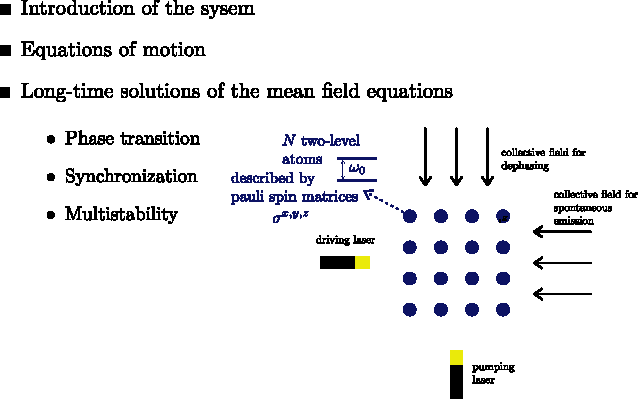
\includegraphics[width=\textwidth]{pictures/outline2.pdf}
% % \footnote{\cite{mattes_entangled_2023}}
% \end{frame}
% \subsection{Introduction of the system}
% \begin{frame}{System setup}
% \vspace*{-1.2cm}
% \hspace*{-0.9cm}
%     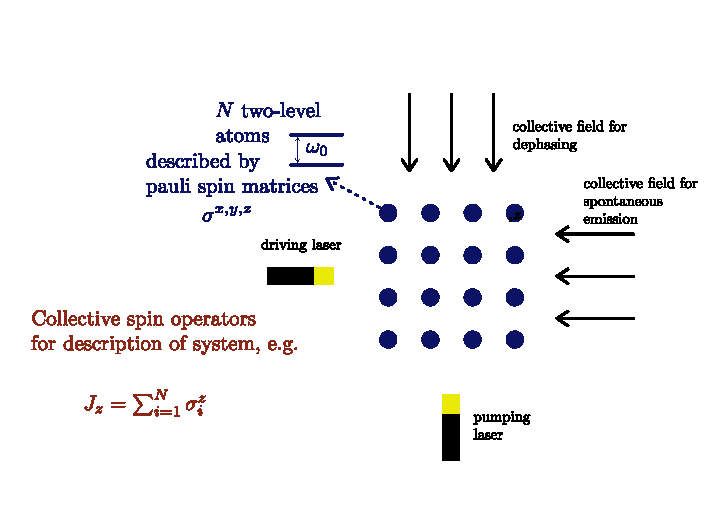
\includegraphics{pictures/lattice.pdf}
% \end{frame}


% \begin{frame}{Composition of the coupling}
% % \vspace*{-0.8cm}
% \hspace*{-0.5cm}
%     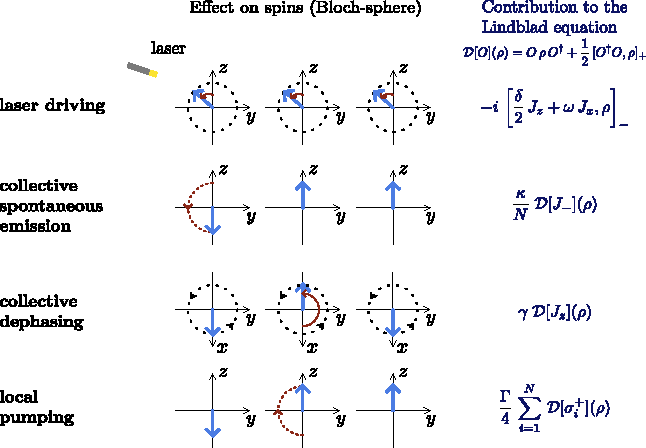
\includegraphics{pictures/couplings4.pdf}
% \end{frame}
% \subsection{Equations of motion}
% \begin{frame}{Equations of motion}

% \textbf{Lindblad equation:}
% \begin{align*}
%     \frac{\diff \rho}{\diff t}&= - \left[\frac{\delta}{2}\,J_z+\omega\,J_x,\rho\right]_-+\frac{\kappa}{N}\,\mathcal{D}[J_-](\rho)+\gamma\,\mathcal{D}[J_z](\rho)+\frac{\Gamma}{4}\,\sum_{i=1}^N\mathcal{D}[\sigma_i^+](\rho)\\\\
%     \text{with}\quad \mathcal{D}[O](\rho)&=O\,\rho \,O^\dagger-\half\,[O^\dagger O,\rho]_+
% \end{align*}
% \textbf{Mean field equations of motion for spin $m_\alpha=\braket{J_\alpha}/N$:}
% \begin{align*}
%     \dt m_x &= -\frac{\delta}{2}\,m_y-\half\,(\gamma+\Gamma)\,m_x+\kappa\,m_x m_z\notag\\
%     \dt m_y &= \frac{\delta}{2}\,m_x-\omega\,m_z-\half\,(\gamma+\Gamma)\,m_y+\kappa\,m_y m_z\notag\\
%     \dt m_z &= \omega\,m_y - \kappa\,(m_x^2+m_y^2)+\half\Gamma-\Gamma\,m_z\label{eq:mean_field}
% \end{align*}
% \end{frame}





% %%%%%%%%%%%%%%%%%%%%%%%%%%%%%%%%%%%%%%%%%%%%%%%%%%%%%%%%%%%%%

\end{document}
